\documentclass{article}

\usepackage[UTF8]{ctex}
\usepackage{placeins}
\usepackage{graphicx}
\usepackage{listings}
\usepackage{xcolor} % 添加 xcolor 宏包
\lstset{ %
language=matlab,                % choose the language of the code
basicstyle=\footnotesize,       % the size of the fonts that are used for the code
numbers=left,                   % where to put the line-numbers
numberstyle=\footnotesize,      % the size of the fonts that are used for the line-numbers
stepnumber=1,                   % the step between two line-numbers. If it is 1 each line will be numbered
numbersep=5pt,                  % how far the line-numbers are from the code
backgroundcolor=\color{white},  % choose the background color. You must add \usepackage{color}
showspaces=false,               % show spaces adding particular underscores
showstringspaces=false,         % underline spaces within strings
showtabs=false,                 % show tabs within strings adding particular underscores
frame=single,           % adds a frame around the code
tabsize=2,          % sets default tabsize to 2 spaces
captionpos=b,           % sets the caption-position to bottom
breaklines=true,        % sets automatic line breaking
breakatwhitespace=false,    % sets if automatic breaks should only happen at whitespace
escapeinside={\%*}{*)}          % if you want to add a comment within your code
}
\title{hw03\_MATLAB}
\author{3220103167 缪晨轩}
\date{\zhdate{2024/3/17}}

\begin{document}

\maketitle
    \section*{59(a)}
        
        \begin{lstlisting}[caption={题59(a)MATLAB代码}, label={lst:matlab}]
            syms t n a;
            T = 4; % 周期
            w0 = 2 * pi / T; % 基本角频率

            % 定义矩形波函数
            f_t = a * heaviside(t + 1) * heaviside(1 - t) + 0 * (heaviside(t + 2) - heaviside(t - 1));

            % 计算傅里叶系数
            Cn = (1 / T) * int(f_t * exp(-1i * n * w0 * t), t, -T/2, T/2);
            C0 = (1 / T) * int(f_t, t, -T/2, T/2);

            % 替换参数 a 的具体值(假设 a = 0.5)
            a_val = 0.5;
            Cn_val = subs(Cn, a, a_val);
            C0_val = subs(C0, a, a_val);

            % 显示傅里叶系数的数值结果
            disp(['Cn: ', char(simplify(Cn_val))]);
            disp(['C0: ', char(simplify(C0_val))]);

        \end{lstlisting}
        Answer: \[a_0 = \frac{1}{4}\]
        \[a_n = \frac{{\sin \left( {\frac{{n\pi }}{2}} \right)}}{{2n\pi }}\]
        \[b_n = 0\]

    \section*{59(b)}
        \begin{lstlisting}[caption={题59(b)MATLAB代码}, label={lst:matlab}]
            syms t n m;
            m = pi;
            T = 2 * pi / m; % 信号的周期

            % 定义原始信号
            f_t = sin(m * t);

            % 定义滤波器
            filtered_f_t = (1/2) * (f_t + abs(f_t)); % 滤波器只保留信号的正值部分

            % 计算滤波后信号的傅里叶系数
            a0 = (2 / T) * int(filtered_f_t, t, 0, T/2); % 直流分量
            an = (2 / T) * int(filtered_f_t * cos(n * 2 * pi / T * t), t, 0, T/2); % 正弦项系数
            bn = (2 / T) * int(filtered_f_t * sin(n * 2 * pi / T * t), t, 0, T/2); % 余弦项系数

            % 显示傅里叶系数的符号表达式
            disp(['a0:', char(simplify(a0))]);
            disp(['an:', char(simplify(an))]);
            disp(['bn:', char(simplify(bn))]);
        \end{lstlisting}
        Answer: \[{a_0} = \frac{2}{\pi }\]
                \[{a_n} = \left\{ {\begin{array}{*{20}{c}}
                0&{n =  - 1 \vee n = 1} \\ 
                { - \frac{{2\cos {{\left( {\frac{{\pi n}}{2}} \right)}^2}}}{{\pi \left( {{n^2} - 1} \right)}}}&{n \ne  - 1 \wedge n \ne 1} 
                \end{array}} \right.\]
                \[{b_n} = \left\{ {\begin{array}{*{20}{c}}
                    {\begin{array}{*{20}{c}}
                    {\frac{1}{2}}&{n = 1} 
                  \end{array}} \\ 
                    {\begin{array}{*{20}{c}}
                    { - \frac{1}{2}}&{n =  - 1} 
                  \end{array}} \\ 
                    {\begin{array}{*{20}{c}}
                    { - \frac{{\sin (\pi n)}}{{\pi ({n^2} - 1)}}}&{n \ne  - 1 \wedge n \ne 1} 
                  \end{array}} 
                  \end{array}} \right.\]
    \section*{61(1)}
        \begin{lstlisting}[caption={题61(1)MATLAB代码}, label={lst:matlab}]
            syms t w;
            f_t = exp(-1i * w * t) * dirac(t - 2); %原信号
            F_w = fourier(f_t, t, w); %计算傅里叶变换
            F_w_simplified = simplify(F_w);
            disp(F_w_simplified)

        \end{lstlisting}
        Answer: \[\exp \left( { - 4iw} \right)\]
    \section*{61(2)}
        \begin{lstlisting}[caption={题61(2)MATLAB代码}, label={lst:matlab}]
            syms t w;
            f_t = sign(2*t^2 - 4); % 定义函数 sgn(2t^2-4)
            F_w = fourier(f_t, t, w); % 计算傅里叶变换
            F_w_simplified = simplify(F_w);
            disp(F_w_simplified) 

        \end{lstlisting}
        Answer: 
            \begin{figure}[h]
                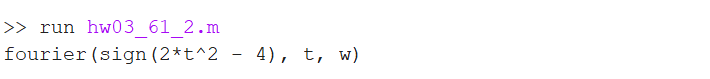
\includegraphics{hw03_61_2.png}
            \end{figure}
            \FloatBarrier
            Actually it doen't satisfy the condition of Fourier Transform.
    \section*{61(3)}
        \begin{lstlisting}[caption={题61(3)MATLAB代码}, label={lst:matlab}]
            syms t w;
            f_t = exp(-5 * t) * heaviside(t + 2); % 定义函数 e^(-5t)*u(t+2)
            F_w = fourier(f_t, t, w); % 计算傅里叶变换
            F_w_simplified = simplify(F_w);
            disp(F_w_simplified) 

        \end{lstlisting}
        Answer: \[\frac{{\exp \left( {10 + 2iw} \right)}}{{5 + iw}}\]
    \section*{61(4)}
        \begin{lstlisting}[caption={题61(4)MATLAB代码}, label={lst:matlab}]
            syms t w;

            ut_shifted = heaviside(t - 1); % t-1的单位阶跃函数

            Fw = fourier(ut_shifted, t, w); % 计算傅里叶变换

            Fw_simpilified = simplify(Fw);
            disp(Fw_simpilified) 

        \end{lstlisting}
        Answer: \[\pi \delta \left( w \right) - \frac{{\exp \left( { - iw} \right)i}}{w}\]


\end{document}
